\documentclass[12pt]{article}

\usepackage{amsmath,amsthm,amsfonts,amssymb,amsxtra}
\usepackage{multicol}
\usepackage{pgf,tikz}
\usetikzlibrary{arrows}
\renewcommand{\theenumi}{(\alph{enumi})} 
\renewcommand{\labelenumi}{\theenumi}

\pagestyle{empty}
\setlength{\textwidth}{7in}
\setlength{\oddsidemargin}{-0.5in}
\setlength{\topmargin}{-1.0in}
\setlength{\textheight}{9.5in}

\theoremstyle{definition}
\newtheorem{problem}{Problem}

\newcommand{\sectionlinetwo}[2]{%
  \nointerlineskip \vspace{.5\baselineskip}\hspace{\fill}
  {\color{#1}
    \resizebox{0.5\linewidth}{2ex}
    {{%
        {\begin{tikzpicture}
            \node  (C) at (0,0) {};
            \node (D) at (9,0) {};
            \path (C) to [ornament=#2] (D);
          \end{tikzpicture}}}}}%
  \hspace{\fill}
  \par\nointerlineskip \vspace{.5\baselineskip}
}

\makeatletter
\newcommand*{\radiobutton}{%
  \@ifstar{\@radiobutton0}{\@radiobutton1}%
}
\newcommand*{\@radiobutton}[1]{%
  \begin{tikzpicture}
    \pgfmathsetlengthmacro\radius{height("X")/2}
    \draw[radius=\radius] circle;
    \ifcase#1 \fill[radius=.6*\radius] circle;\fi
  \end{tikzpicture}%
}
\makeatother

\begin{document}

\noindent{\large\bf MATH 122}\hfill{\large\bf Exam \#1.}\hfill{\large\bf  Fall 2018}\hfill{\large\bf Page 1/7}\hrule

\bigskip
\begin{center}
  \begin{tabular}{|ll|}
    \hline & \cr
             {\bf Name: } & \makebox[12cm]{\hrulefill}\cr & \cr
                                                            {\bf VIP ID:} & \makebox[12cm]{\hrulefill}\cr & \cr
                                                                                                            \hline
  \end{tabular}
\end{center}
\begin{itemize}
\item Write your name and VIP ID in the space provided above.
\item The test has seven (7) pages, including this one.
\item Each question is worth 5 points. 
\item No books, or notes may be used on this test.
\item An approved calculator may be used on this test.
\end{itemize}
\hrule

\newpage

%%%%%%%%%%%%%%%%%%%%%%%%%%%%%%%%%%%%% Page 2
\noindent{\large\bf MATH 122}\hfill{\large\bf Exam \#1.}\hfill{\large\bf  Fall 2018}\hfill{\large\bf Page 2/7}\hrule

\bigskip
\begin{problem}[5 pts]
  The following table gives the sales of the medicinal herb \textit{saw palmetto}, in millions of dollars, for several
  different years: 
  \begin{center}
    \begin{tabular}{l||c|c|c|c|c|}
      Year & 1997 & 1998 & 1999 & 2000 & 2001 \\
      \hline
      Sales (million dollars) & 85 & 107 & 116 & 122 & 123
    \end{tabular}
  \end{center}
  The average rate of change of sales over the period 1998 to 2000 is:
  \begin{itemize}
  \item[\radiobutton] 3.5 million dollars/year
  \item[\radiobutton] 3.5 million dollars
  \item[\radiobutton] 7.5 million dollars/year
  \item[\radiobutton] 7.5 million dollars
  \item[\radiobutton] 9.5 million dollars/year
  \item[\radiobutton] 9.5 million dollars
  \item[\radiobutton] 15 million dollars/year
  \item[\radiobutton] 15 million dollars
  \end{itemize}
\end{problem}
\hrule

\begin{problem}[5 pts]
  Find the domain of the function $f(x) = \dfrac{5x+3}{4x-1}$

  \vspace{3cm}
\end{problem}
\hrule

\begin{problem}[5 pts]
  A car rental company offers two plans for renting a car.  The first plan charges \$32 per day and 16 cents per
  mile.  The second plan charges \$50 per day with free unlimited mileage.  How many miles are needed for the second
  plan to save us money?
\end{problem}

\newpage

%%%%%%%%%%%%%%%%%%%%%%%%%%%%%%%%%%%%% Page 3
\noindent{\large\bf MATH 122}\hfill{\large\bf Exam \#1.}\hfill{\large\bf  Fall 2018}\hfill{\large\bf Page 3/7}\hrule

\bigskip
\begin{problem}[5 pts]
  Write an equation for the quadratic equation graphed:
  \begin{multicols}{2}
    \begin{tikzpicture}[scale=0.75]
      \draw[gray, ultra thin, step=1] (-5,-1) grid (5,9);
      \draw[thick,<->] (-5,0) -- (5,0);
      \draw[thick,<->] (0,-1) -- (0,9);
      \draw (0,-1) parabola bend (2,7) (4,-1);
      \draw[fill=black] (0,-1) circle (3pt) node[left]{$(0,-1)$};
      \draw[fill=black] (2,7) circle (3pt) node[above]{$(2,7)$};
    \end{tikzpicture}

    \begin{itemize}
    \item[\radiobutton] $y=(x-2)^2 - 3$
    \item[\radiobutton] $y=(x+1)^2 +2$
    \item[\radiobutton] $y=-2(x-2)^2 + 7$
    \item[\radiobutton] $y=-3(x+1)^2 + 2$
    \end{itemize}
  \end{multicols}
\end{problem}
\hrule

\begin{problem}[5 pts]
  The cost in dollars to produce $q$ tons of an item is given by the function $C = 100 + 20q$. What are the units of
  the 20? 
  \begin{itemize}
  \item[\radiobutton] Dollars
  \item[\radiobutton] Tons
  \item[\radiobutton] Dollars/Tons
  \item[\radiobutton] Tons/Dollars
  \end{itemize} 
\end{problem}
\hrule

\begin{problem}[5 pts]
  It costs a total of $C$ dollars to extract $T$ tons of ore from a copper mine. If $C$ is a linear function of $T$, the
  units of the slope of the line are: 
  \begin{itemize}
  \item[\radiobutton] Tons
  \item[\radiobutton] Dollars
  \item[\radiobutton] Tons/dollar
  \item[\radiobutton] Dollars/ton
  \end{itemize}
\end{problem}
\hrule

\begin{problem}[5 pts]
  Find the equation of a line that passes through $(2,4)$ and $(4,10)$.
  \begin{itemize}
  \item[\radiobutton] $y=4+3(x-2)$
  \item[\radiobutton] $y=8-\tfrac{1}{3}(x-8)$
  \item[\radiobutton] $y+3=-\tfrac{3}{2}x$
  \item[\radiobutton] $y=4+\tfrac{4}{5}x$
  \end{itemize}
\end{problem}
\newpage

%%%%%%%%%%%%%%%%%%%%%%%%%%%%%%%%%%%%% Page 4
\noindent{\large\bf MATH 122}\hfill{\large\bf Exam \#1.}\hfill{\large\bf Fall 2018}\hfill{\large\bf Page 4/7}\hrule

\bigskip
\begin{problem}[5 pts]
  The graph below is a representation of which of the following functions?
  \begin{multicols}{2}
    \begin{tikzpicture}[scale=0.4]
      \draw[gray, ultra thin, step=1] (-4,-3) grid (11,12);
      \draw[thick, <->] (-4,0) -- (11,0);
      \draw[thick, <->] (0,-3) -- (0,12);
      \draw (-2,12) -- (3,-3);
      \draw[fill=black] (0,6) circle (5pt) node[left]{$(0,6)$};
      \draw[fill=black] (2,0) circle (5pt) node[above right]{$(2,0)$};
    \end{tikzpicture}
    
    \begin{itemize}
    \item[\radiobutton] $y=-3x+2$
    \item[\radiobutton] $y=6x-2$
    \item[\radiobutton] $y=6x+6$
    \item[\radiobutton] $y=-3x+6$
     \end{itemize}
  \end{multicols}
\end{problem}
\hrule

\begin{problem}[5 pts]
  When a person goes into shock, the cardiac output, in liters of blood per minute, decreases. One person’s cardiac output
  is 12 liters per minute when the person first goes into shock, and decreases by 2 liters per minute every hour that the
  person is in shock. Write a formula for cardiac output $C$ as a function of $t$, the time in hours since a person first
  went into shock. 
  \begin{itemize}
  \item[\radiobutton] $C = 12 - 2t$
  \item[\radiobutton] $t = 12 - 2C$
  \item[\radiobutton] $C = -2 + 12t$
  \item[\radiobutton] $t = -2 + 12t$
  \item[\radiobutton] $C = 12 + 2t$
  \item[\radiobutton] $t = 12 + 2C$
  \end{itemize}
\end{problem}
\hrule

\begin{problem}[5 pts]
  Solve the following inequality:
  \begin{equation*} (x-5)(x+1)^2 > 0 \end{equation*}
\end{problem}

\newpage

%%%%%%%%%%%%%%%%%%%%%%%%%%%%%%%%%%%%% Page 5
\noindent{\large\bf MATH 122}\hfill{\large\bf Exam \#1.}\hfill{\large\bf  Fall 2018}\hfill{\large\bf Page 5/7}\hrule

\bigskip

\begin{problem}[5 pts]
  The concentration of a pollutant in a lake was 85 parts per million (ppm) in the year 2017 and is increasing at a rate of 4.6\% each
  year.  When will the concentration of pollutant reach 100 ppm?

  \vspace{8cm}

\end{problem}
\hrule

\begin{problem}[5 pts]
  Indicate whether the following are power functions. In case they are, find a suitable constant of proportionality $C$,
  and power $r$ so you could write those functions in the form $f(x) = Cx^r$. 
  \begin{center}
    \begin{tabular}{|c|c|c|c|}
      \hline
      $f(x)$ & Is it a power function? & $C$ & $r$ \\
      \hline
      \hline
             &&& \\
      $5\sqrt{x}$ &&\hspace{1cm} & \hspace{1cm} \\
             &&& \\
      \hline
             &&& \\
      $17^x$ &&& \\
             &&& \\
      \hline
             &&& \\
      $(3x^5)^2$ &&& \\
             &&& \\
      \hline
             &&& \\
      $\dfrac{5}{2\sqrt{x}}$ &&& \\
             &&& \\
      \hline
             &&& \\
      $\pi$ &&& \\
             &&& \\
      \hline
    \end{tabular}
  \end{center}
\end{problem}
\newpage


%%%%%%%%%%%%%%%%%%%%%%%%%%%%%%%%%%%%% Page 6
\noindent{\large\bf MATH 122}\hfill{\large\bf Exam \#1.}\hfill{\large\bf  Fall 2018}\hfill{\large\bf Page 6/7}\hrule

\bigskip
\begin{problem}[5 pts]
  Evaluate $f(-2)$ for $f(x) = 4-\sqrt[3]{x-2}$.

  \vspace{2cm}
\end{problem}
\hrule

\begin{problem}[5 pts]
  Solve $f(x)=4$ for $f(x) = 4-\sqrt[3]{x-2}$.

  \vspace{2cm}
\end{problem}
\hrule

\begin{problem}[5 pts]
  Evaluate $f(7)$ for the function $f$ given as a table below.
  \begin{equation*}
    \begin{array}{|l|r|r|r|r|r|r|r|r|r|r|}
      \hline
      \boldsymbol{x} & 0 & 1 & 2 & 3 & 4 & 5 & 6 & 7 & 8 & 9 \\ \hline
      \boldsymbol{f(x)} & 62 & 8 & 7 & 38 & 86 & 73 & 70 & 39 & 75 & 34 \\ \hline
    \end{array}
  \end{equation*}

  \vspace{1cm}
\end{problem}
\hrule

\begin{problem}[5 pts]
  Solve $f(x)=7$ for the function $f$ given as a table below.
  \begin{equation*}
    \begin{array}{|l|r|r|r|r|r|r|r|r|r|r|}
      \hline
      \boldsymbol{x} & 0 & 1 & 2 & 3 & 4 & 5 & 6 & 7 & 8 & 9 \\ \hline
      \boldsymbol{f(x)} & 62 & 8 & 7 & 38 & 86 & 73 & 70 & 39 & 75 & 34 \\ \hline
    \end{array}
  \end{equation*}

  \vspace{1cm}
\end{problem}
\hrule

\begin{problem}[5 pts]
  Solve for $t$ in the equation $200 = 30e^{0.15t}$

  \vspace{4cm}
\end{problem}
\hrule

\begin{problem}[5 pts]
  Solve for $x$ in the equation $4^{2x-3} = 44$

\end{problem}
\newpage 


%%%%%%%%%%%%%%%%%%%%%%%%%%%%%%%%%%%%% Page 7
\noindent{\large\bf MATH 122}\hfill{\large\bf Exam \#1.}\hfill{\large\bf  Fall 2018}\hfill{\large\bf Page 7/7}\hrule

\bigskip
\begin{problem}[5 pts]
  Sales at a company are changing according to the formula $S = 1000 (0.82)^t$ , where $S$ is sales in thousands of
  dollars and $t$ is measured in years. Sales at this company are: 
  \begin{itemize}
  \item[\radiobutton] Increasing by 82\% per year
  \item[\radiobutton] Increasing by 82 thousand dollars per year
  \item[\radiobutton] Decreasing by 82\% per year
  \item[\radiobutton] Decreasing by 82 thousand dollars per year
  \item[\radiobutton] Increasing by 18\% per year
  \item[\radiobutton] Increasing by 18 thousand dollars per year
  \item[\radiobutton] Decreasing by 18\% per year
  \item[\radiobutton] Decreasing by 18 thousand dollars per year
  \end{itemize} 
\end{problem}
\hrule

\begin{problem}[5 pts]
  The amount, $A$ (in mg), of a drug in the body is 25 when it first enters the system is decreases by 12\% each hour. A
  possible formula for $A$ as a function of $t$, in hours after the drug enters the system, is:
  \begin{itemize}
  \item[\radiobutton] $A=25+12t$
  \item[\radiobutton] $A=25-12t$
  \item[\radiobutton] $A=25+0.12t$
  \item[\radiobutton] $A=25-0.12t$
  \item[\radiobutton] $A=25(0.12)^t$
  \item[\radiobutton] $A=25(0.88)^t$
  \item[\radiobutton] $A=25(1.12)^t$
  \item[\radiobutton] $A=25(1.88)^t$
  \item[\radiobutton] $A=25(-0.12)^t$
  \end{itemize}
\end{problem}

\end{document}
